%% Original Template Author: Robin Turner, Adapted from the IEEE peer review template
%% by Luca Dalmasso
%% 

\documentclass[a4paper]{report}
\usepackage{cite} % Tidies up citation numbers.
\usepackage{url} % Provides better formatting of URLs.
\usepackage[utf8]{inputenc} % Allows Turkish characters.
\usepackage{booktabs} % Allows the use of \toprule, \midrule and \bottomrule in tables for horizontal lines
\usepackage{graphicx}
\usepackage{xcolor}
\usepackage[ruled,vlined,linesnumbered]{algorithm2e}
% Corrects some bad hyphenation
\hyphenation{} 



\begin{document}
\title{GPU programming \\ LeNet-1 Project Report}
\author{Dalmasso Luca\\
        Embedded Systems master degree\\
        Politecnico of Turin
        }

\date{01/07/2022}

% make the title area
\maketitle
\tableofcontents
\listoffigures
\listoftables

%\end{titlepage}

%\IEEEpeerreviewmaketitle
\begin{abstract}
This project consists in developing the LeNet-1 Convolutional Neural Network with the aim of speeding it up in a GPU through the CUDA programming language.\\
In this report is presented one possible implementation of the CNN on the GPU that starts from a very naïve version of the algorithm and shows what are the optimisations that were implemented in order to get better performances and better usage of the GPU resources.

\end{abstract}

\section{Introduction}
In the domain of Machine Learning, Convolutional Neural Networks (CNNs) are particular class of  Depp Learning algorithms specifically designed to process pixel data and so  widely used for image classification and object recognition.
The LeNet-1 is a CNN architecture introduced in 1998 by Yann LeCun and other researchers as an attempt to classify 2D images, in particular with the purpose of recognising handwritten digits in ZIP codes.

%%%CAP 2 BACKGROUND %%%%%
\section{Background}
A very general architecture of a CNN is the one showed in Figure 1 where it is possible to see that, from a general point of view, a CNN is a sequence of layers.
Each layer is composed of a set of feature maps and each feature map is processed by some mathematical operations and transformed into another feature map and so on.
The number of layers as well as the number of feature maps of each layer and their size really depends on what kind of image you would like to classify and what kind of accuracy you need and also how many resources you have.\\
Layers in a CNN are divided into three categories:
\begin{enumerate}
\item Input Layer: is the first layer of a CNN and it is the input image that needs to be classified.
 An example of input layer can be the robot in the Figure 1 .
\item Hidden layer: any middle layer in a CNN is also called hidden layer and they are a set of feature maps.
They are called hidden because their inputs and outputs are masked by convolutions , activation function and pooling or subsampling functions.
Each hidden layer is used as an input of the next hidden layer until the last one, which is flattened and processed to become the output layer.
An example of hidden layer can be the first four feature maps of the Figure 1 that are obtained starting from the input image convolved with four different filters.
\item Output layer: contains the results of the classification.
\end{enumerate}

\begin{figure}[h]
\centering
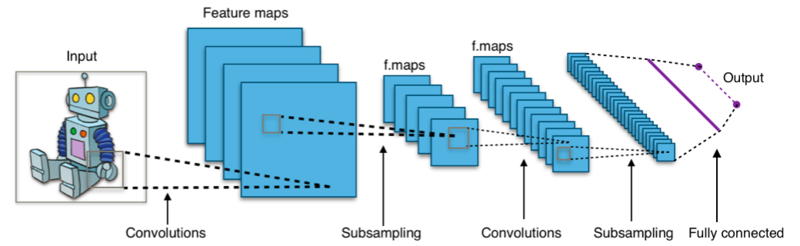
\includegraphics[width=0.8\columnwidth]{docs/Typical_cnn.png} 
\caption{Typical CNN}
\label{fig_typicalCNN}
\end{figure}

The three operations mentioned before (convolution, activation function and pooling) are the set of mathematical ingredients that are used in any CNN to process and classify images.


\subsection{Convolution}
given an image \( I \epsilon R^{n \cdot m}  \) and a filter  \( K \epsilon R^{k \cdot k}  \) the resulting pixel of this operation \( I_{x,y} * K \) (which is a 2D convolution) is the result of the following equation:
\begin{equation} 
\label{conv1}
Ic_{(x,y)} = I_{x,y} * K = \sum_{u=-k/2}^{k/2}\sum_{v=-k/2}^{k/2}K_{u,v} \cdot I_{x-u,y-v}
 \end{equation}
The equation (1) requires to flip the filter K and to center it on the target pixel \( I_{x,y} \), if you consider the filter as a set of weights then the resulting pixel \( Ic_{(x,y)} \) is just a weighted sum of the input pixel \( I_{x,y} \) and the surrounding ones.\\
Due to the fact that in a CNN the filter can be considered already inverted and not all input pixels are convoluted but only those in the central portion of the image where the filter doesn't go out of border: \[x \in [k/2,m-k/2], y \in [k/2, n-k/2] \] the operation can be simplified as a standard dot product:
\begin{equation}
\label{conv2}
Ic_{(x,y)} = \sum_{u=0}^{k}\sum_{v=0}^{k}K_{u,v} \cdot I_{x+u,y+v}
 \end{equation}
Just to be clear, the following example makes use of the equation (1) where for simplicity the filter K is the identity filter (in this case the inverted version K' is the same K):
\[
I
\left(
\begin{array}{ccccccc}
  1&   2&  3&   4&   5&   6  \\
  7&   8&  9&  10&  11& 12         \\
  13&   14& 15& 16& 17& 18  \\
  19&   20& 21& 22& 23& 24 \\
  25&   26& 27& 28& 29& 30  \\
  31&   32& 33& 34& 35& 36 \\
\end{array}
\right)
*
K
\left(
\begin{array}{ccc}
  0&   0&  0 \\
  0&   1&  0 \\
  0&   0& 0 
\end{array}
\right)
=
\left(
\begin{array}{ccccccc}
  1&   2&  3&   4&   5&   6  \\
  7&   8&  9&  10&  11& 12         \\
  13&   14& 15& 16& 17& 18  \\
  19&   20& 21& 22& 23& 24 \\
  25&   26& 27& 28& 29& 30  \\
  31&   32& 33& 34& 35& 36 \\
\end{array}
\right)
\]

The following example makes use of the equation (2) with the same I, K:
\[
I
\left(
\begin{array}{ccccccc}
  1&   2&  3&   4&   5&   6  \\
  7&   8&  9&  10&  11& 12         \\
  13&   14& 15& 16& 17& 18  \\
  19&   20& 21& 22& 23& 24 \\
  25&   26& 27& 28& 29& 30  \\
  31&   32& 33& 34& 35& 36 \\
\end{array}
\right)
*
K
\left(
\begin{array}{ccc}
  0&   0&  0 \\
  0&   1&  0 \\
  0&   0& 0 
\end{array}
\right)
=
\left(
\begin{array}{ccccc}
  8&  9&  10&  11 \\
  14& 15& 16& 17  \\
  20& 21& 22& 23 \\
  26& 27& 28& 29 \\
\end{array}
\right)
\]

This is the formula used to compute the output matrix's size Os starting from input matrix's size Is and filter's size Ks:
\begin{equation} 
\label{outsize}
Os = Is - Ks +1
 \end{equation}

\subsection{Activation Function}
The activation function, sometimes also called transfer function, defines how the weighted sum of the input (so the result of a convolution) is transformed into an output value.\\
There are different types of activation functions and usually many of them are nonlinear functions,  and the choice of which activation function to use can really affects the performances and the capabilities of a neural network.\\
Typically every pixel after being convoluted is also activated, this operation is performed by the convolution layers.\\
Without going into many details, the LeNet-1 makes use of the Sigmoid function which is the following nonlinear function:
\begin{equation} 
\label{outsize}
S(x) = \frac{1}{1+e^{-x}}
 \end{equation}
 
\begin{figure}[h]
\centering
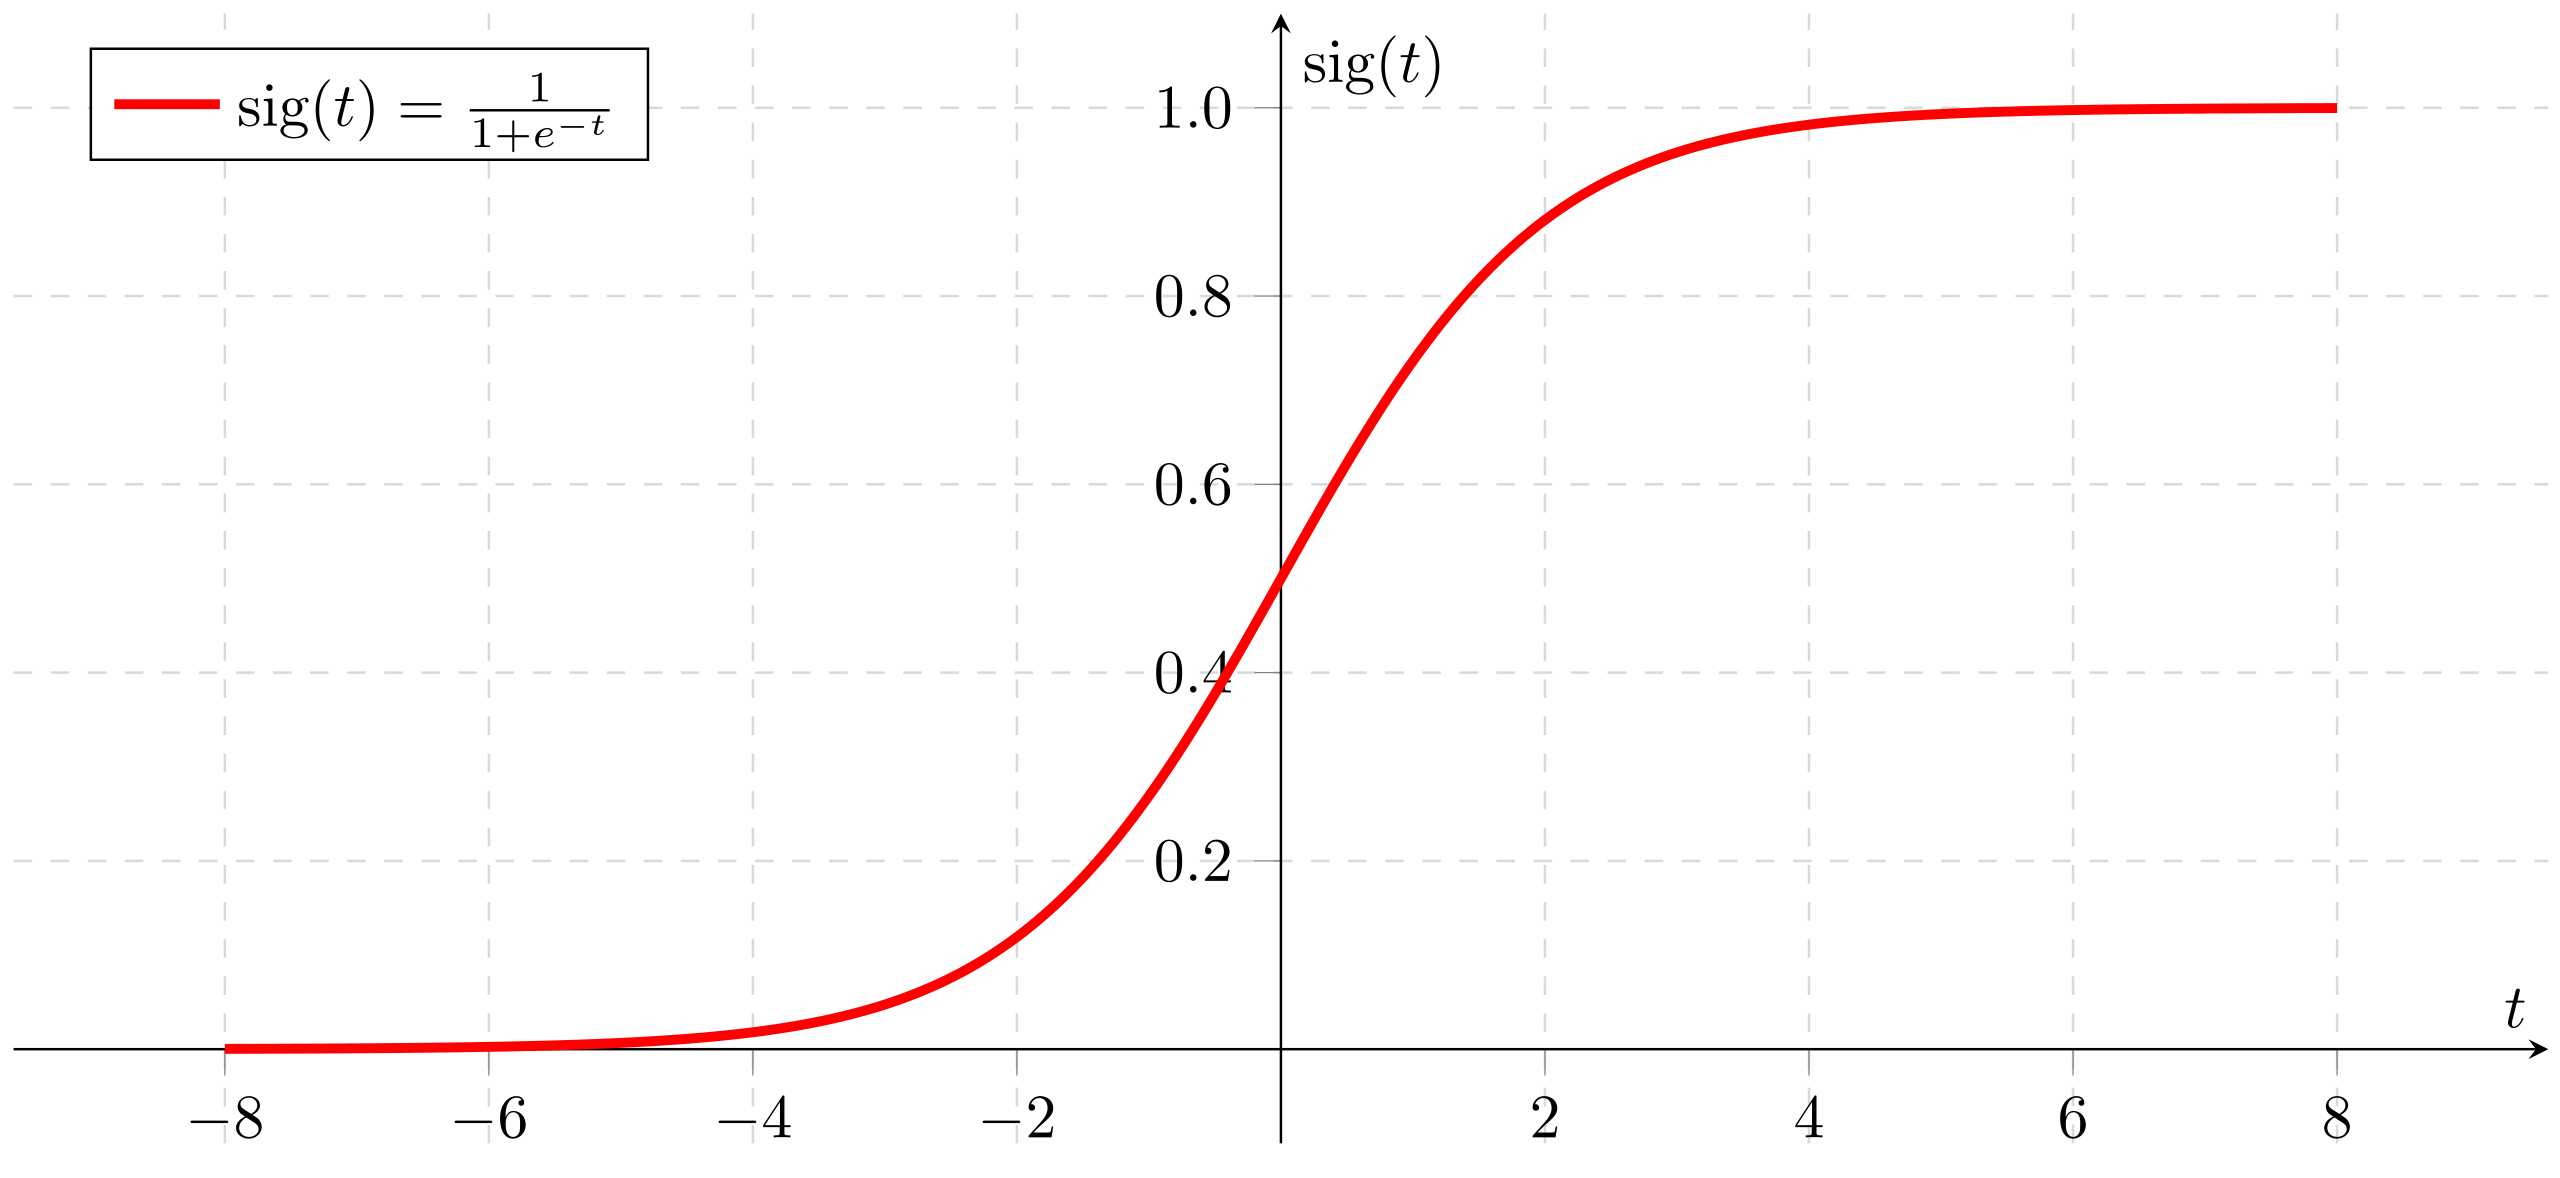
\includegraphics[width=0.8\columnwidth]{docs/sigmoid.png} 
\caption{Sigmoid activation function}
\label{fig_sigmoid}
\end{figure}
 

\subsection{Pooling Function}
Another widely used operation in a CNN is the Pooling function also called Subsampling function.\\
Pooling is a sample-based discretisation process with the aim of down-sample an input representation (image, hidden-layer, generic matrix, etc) and so reducing it's dimensionality.\\
The basic procedure of pooling is very similar to the convolution operation. You select a filter, you slide it over the input representation and you obtain a new output representation.\\
In this case the most commonly used filter size is 2x2 and the filter is slid over the input pixels with a stride of 2.\\\\\\\\
There are several approaches to pooling, the most commonly used are the following two:

\begin{itemize}  
\item Max Pooling: \\
the filter simply selects the maximum pixel value in the 2x2 region\\
example:\\
\[
\left(
\begin{array}{ccccc}
  8&  9&  10&  11 \\
  14& 15& 16& 17  \\
  20& 21& 22& 23 \\
  26& 27& 28& 29 \\
\end{array}
\right)
\mapsto
\left(
\begin{array}{cc}
  15&  17  \\
  27& 29
\end{array}
\right)
\]
\item Average Pooling: \\
in this case the pooling works by calculating the average value of the pixels in the 2x2 region\\
example:\\
\[
\left(
\begin{array}{ccccc}
  8&  9&  10&  11 \\
  14& 15& 16& 17  \\
  20& 21& 22& 23 \\
  26& 27& 28& 29 \\
\end{array}
\right)
\mapsto
\left(
\begin{array}{cc}
  11.5&  13.5  \\
  23.5& 25.5
\end{array}
\right)
\]
\end{itemize}

Right now, many implementations use max pooling because it is less expensive from a computationally point of view and it can helps in speeding up the CNN.


%%%CAP 3 PROJECT DESCRIPTION %%%%%
\section{LeNet-1 Architecture}
Now that all the mathematical basics were briefly introduced the discussion can finally introduce the forward propagation algorithm of the LeNet-1 CNN.\\
\begin{figure}[!h]
\centering
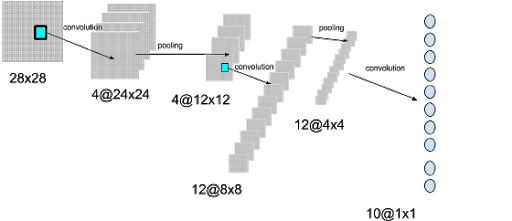
\includegraphics[width=0.8\columnwidth]{docs/LeNet1.png} 
\caption{Anatomy of the LeNet-1}
\label{fig_lenet}
\end{figure}

From Figure 3 it is possible to observe that, starting from the input layer, the overall architecture is composed of 3 convolutional layers and 2 pooling layers for a total amount of 4 hidden layers and a final output layer.
\begin{enumerate}
\item Input Layer: \\
consists of a 28x28 image that represents the first 784 input neurons.
\item First Hidden layer: \\
First convolutional layer composed of four 24x24 feature maps that forms a group of 2304 neurons.
\item Second Hidden layer:\\
First average pooling layer composed of four 12x12 feature maps that forms a group of 576 neurons.
\item Third Hidden layer:\\
Second convolutional layer composed of twelve 8x8 feature maps that forms a group of 768 neurons.
\item Fourth Hidden layer:\\
Second and last average pooling layer composed of twelve 4x4 feature maps that forms a group of 192 neurons.
\item Output layer:\\
Contains the result of the classification of the input image. This CNN as said in the Introduction is meant to be used to classify digits between 0-9, so the output layer contains the classification on a 10x1 array.
\end{enumerate}


\subsection{Description of the first hidden layer}
Starting from the input image, four filters K1, K2, K3, K4 of size 5x5 (25 weights each) are convoluted to generate the four feature maps.\\
The size of each feature map is 24x24 and can be easily computed with the equation (3) where Is=28 and Ks=5.\\
The visual representation of the first convolutional layer is showed in Figure 4.\\
The values of the first layer are instead given by the following equation:
\begin{equation} 
\label{convLayer}
F^{s}_{x,y} = \sigma (bias + \sum_{u=0}^{4}\sum_{v=0}^{4}K^{s}_{u,v} \cdot I_{x+u,y+v})
 \end{equation}
 \
Where \( F^{s}_{x,y} \) is the (x,y) neuron of the s-th feature, \( \sigma \) is the Sigmoid activation function in the equation (4) that transform the result of convolution (equation (2)) plus a bias term.\\
The remaining parts of the equation are the term \( K^{s}_{u,v} \) that is the (u,v) weight of the s-th filter, and finally \( I_{x+u,y+v} \) is the (x+u,y+v) pixel of the input image.\\\\\\\\
\begin{figure}[!h]
\centering
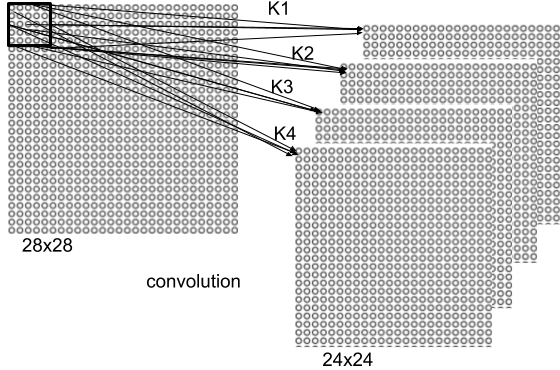
\includegraphics[scale=0.3]{docs/c1.png} 
\caption{First convolutional layer, first hidden layer}
\label{fig_c1}
\end{figure}

\subsection{All layers}
Stated that LeNet-1 has an overall of three convolutional layers and two pooling layers, the network can be described by the following flow:
\[ INPUT \mapsto C1 \mapsto S1 \mapsto C2 \mapsto S2 \mapsto C3 \mapsto OUTPUT \]
Once the input has been convoluted into four feature maps, each feature map is pooled into 4 corresponding feature maps of 12x12 each.\\
In the next layer, the third hidden layer, the convolution is done again by the same equation (5) but this time there are only 3 filters 5x5.
Since the three filters are convoluted on each of the four feature maps, this multiplies the amount of feature maps of the next layer to 12.
Now the new layer is pooled again and by doing that the last hidden layer is created and the size is reduced from 768 to 192 neurons.
Finally we are ready to fully connect the twelve 4x4 features to the output, in this case the convolution is done by using 10 4x4 filters to create the last 10 neurons.\\
The following image can help to understand how the last hidden layer is fully connected to the ouput.
Just consider that Ki is denoted as the i-th filter over the total 10 and Fj as well is the j-th feature map over the total 12. 

\begin{figure}[!h]
\centering
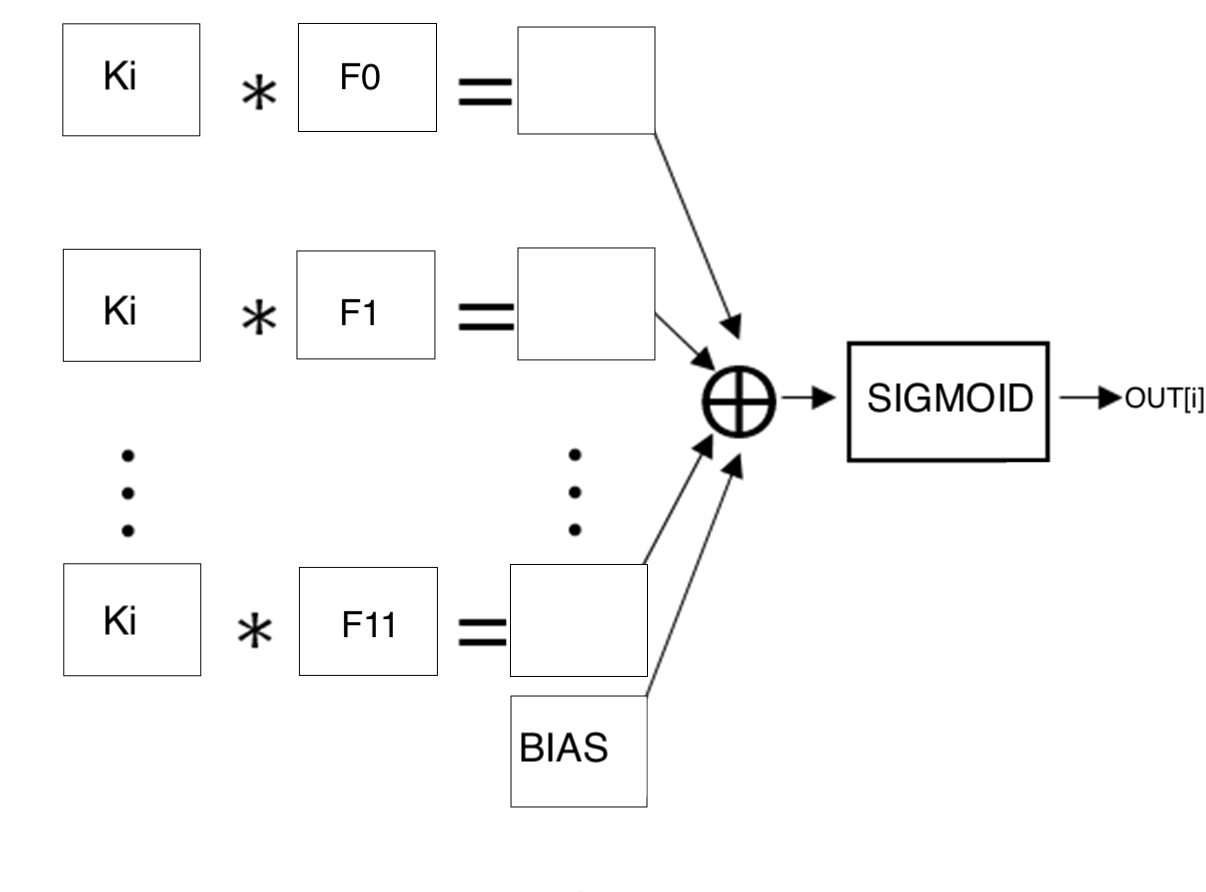
\includegraphics[scale=0.7]{docs/c3.png} 
\caption{Third convolutional layer, Fully connected to output layer}
\label{fig_c3}
\end{figure}

\subsection{Other comments about LeNet}
Even if the architecture of the LeNet-1 CNN is a very simple example without too many hidden layers and features it is important to underline that every forward propagation (every image classification) requires a big set of operations that are sequences of multiplications, additions, divisions and exponentials.
All the mentioned operations repeated for every neuron inside the network will require hundreds of thousands of floating point operation and this render the problem heavy from a computational point of view!

\section{Implementation}
The board used for implementing and testing the forward propagation algorithm is the NVIDIA Jetson Nano.\\
First of all the forward propagation was implemented on the CPU (host) to have a reference benchmark to improve of the algorithm executed serially, then the code was ported on the GPU (device).\\
Concerning the device implementation there are three solution proposed:
\begin{enumerate}
\item heavy usage of global memory, shared memory and constant memory unused.
\item light usage of global memory, all computations in shared memory.
\item soft usage of global memory, all computations in shared memory, filters in constant memory.
\end{enumerate}

\subsection{Host implementation \& serial benchmarks}
The host code is very simple, it serially executes this series of transformations:
\[ Image28x28 \mapsto C1_{4x24x24} \mapsto S1_{4x12x12} \mapsto C2_{12x8x8} \mapsto S2_{12x4x4} \mapsto C3_{10x1x1} \mapsto OUTPUT \]
where \(Ci\) is the i-th convolutional layer , \(Sk\) is the k-th average pooling layer and \( C3_{10x1x1} \) is the last convolutional layer that fully connects to the output.\\

%\subsection{Setup}
 %A specific angle range have been provided to us from the guys building the flap and we had to match that one with our servo, by acting on the dutycycle length in terms of microseconds (900-1480 is the range we found out).
 
%\subsection{Reliability}
%A watchdog has been inserted in the system to avoid stalls in the running application. Basically, if the system stops acquiring and computing the wanted results for more than 5 seconds, it will be forced to reboot.\\
%Furthermore, if the IMU sensor loses the calibration, the input for the PID controller is obtained from the average between the 2 distances measured by ultrasonic sensors at stern, averaged again with that from the one at bow.

%\subsection{Main board peculiarities}
%We worked with an STM32F411RE board, which is considered as high performance, having a 100MHz Cortex-M4, which allowed us to stress the system by reducing the sample rate without having computation losses, at least talking about milliseconds. We then took advantage of the following features provided by the board: a PWM timer for motor control, up to three I2Cs, used to communicate with the IMU, and five SPIs, exploited to communicate with the RFID reader.

%\section{How does the system work}
%The control system is mounted inside the boat, in particular above the drift, as this is point of interest. The two ultrasonic sensors, mounted at stern, are placed on the side wings. 
%We use an RFID reader to configure the system's parameters. Two different cards are read in order to set: target height and sensibility threshold.
%The system maintains one counter for both of them, to modify the settings according to how many times a card was read. 
%The reading is confirmed by a sound produced by a piezoelectric buzzer, which reproduces a different musical note, depending on the parameter we want to change and the currently selected configuration.

%In the following figure is shown the schematic of the connections between board and sensors.\\

%\begin{figure}[!h]
%\centering
%\includegraphics[width=\columnwidth]{interconnections.jpg} 
%\\caption{Connections between board and sensors}
%\\label{fig_sim}
%\\end{figure}

%\All the sensors have been mounted on a 3d printed support, made on purpose to accomodate the microcontroller, the IMU and the RFID reader, as well as the ultrasonic drivers. This "brain" of the system can be easily removed from the moth model, in order to calibrate the IMU, by performing the usual 8 in air around all the 3 different axes; when the calibration status reaches at least a medium value, a sound is emitted and the system can be mounted again in place.

%\\begin{figure}[!h]
%\\centering
%\includegraphics[width=0.8\columnwidth]{3dSupport.jpeg} 
%\\caption{3d printed support}
%\\label{fig_sim}
%\\end{figure}

%\\begin{figure}[!h]
%\\centering
%\includegraphics[width=0.8\columnwidth]{CU.jpg}
%\\caption{Mounted control unit}
%\\end{figure}

%\Finally, a model of the boat has been built to verify the correct behavior of the sensors and servo motor. In particular, it is composed of a foam hull, wooden appendages and a metal mechanism to translate the servo motor movement to the one of the flap.

%\\section{Testing}
%\All the single components have been tested separately to check their functionality and possible integration problems.
%\Concerning the ultrasonic sensors, they have been properly calibrated by means of proper adjustments on the drivers.
%\It is then possible to perform these different tests by acting on proper macros present in the code, like comment removal of \#define WATCHDOG\_TEST to effectively test the watchdog functionality.\\

%\The decision of mounting the ultrasonic sensors on the edges has been adopted also in the real skiff and some tests have been performed to see if the minimum measurable height is guaranteed to be exceeded.

%\\begin{figure}[!h]
%\\centering
%\includegraphics[width=0.8\columnwidth]{keth2.jpg} 
%\\caption{Sensors measurement}
%\\label{fig_sim}
%\\end{figure}

%\The whole system has then been properly checked on a model, to see its correct behavior; all the results can be seen in the proper section.

%\\begin{figure}[!h]
%\\centering
%\includegraphics[width=0.8\columnwidth]{model_of_boat.jpg}
%\\caption{Model of the moth}
%\\end{figure}

%\\section{Results and discussion}

%\The real behavior of the boat has been simulated by physically holding the model at different heights, observing the flap behavior and collecting data.

%\\begin{itemize}  
%\\item Below the target height: \\
%\the flap is oriented fully upwards (dutycycle = 1480), to increase the lift and make the moth fly (see \ref{table:below}).
%\\item Above the target height: \\
%\the flap is oriented fully downwards (dutycycle = 900), to make the moth going down, reducing the lift, avoiding it to take off (see \ref{table:above}).
%\\item Approaching the target height: \\
%\the flap continuously varies its orientation to maintain the target height (see \ref{table:target1}).
%\Another acquisition has been reported to highlight the impact of the spatial orientation of the boat on the height determination (see \ref{table:target2}); in that case we saw that, more o less as expected, the roll angle is correctly weighting the measured distances to determine the flight height.
%\\end{itemize}

%\Pitch and Roll angles are expressed in radiants, the height is in mm and the servomotor's dutycycle is in $\mu$s.\\

%\\begin{table}[!h]
%\\centering
%\\begin{tabular}{|r|r|r|r|r|}
%\\hline
%\\textbf{Time h/m/s/ms} & \textbf{Pitch} & \textbf{Roll} & \textbf{Height} & \textbf{Duty Cycle} \\ \hline
%\15:27:09.401           & -0.28          & 0.02          & 518.88          & 1480.00       \\ \hline
%\15:27:09.436           & -0.25          & 0.04          & 518.55          & 1480.00       \\ \hline
%\15:27:09.511           & -0.27          & 0.00          & 522.42          & 1480.00       \\ \hline
%\15:27:09.600           & -0.26          & -0.01         & 530.57          & 1480.00       \\ \hline
%\15:27:09.646           & -0.24          & -0.02         & 532.81          & 1480.00       \\ \hline
%\\end{tabular}
%\\vspace*{3mm}
%\\caption{Below the target height}
%\\label{table:below}
%\\end{table}

%\\begin{table}[!h]
%\\centering
%\\begin{tabular}{|r|r|r|r|r|}
%\\hline
%\\textbf{Time h/m/s/ms} & \textbf{Pitch} & \textbf{Roll} & \textbf{Height} & \textbf{Duty Cycle} \\ \hline
%\15:26:28.234           & 0.01           & 0.01          & 940.69          & 900.00        \\ \hline
%\15:26:28.317           & 0.00           & 0.02          & 939.86          & 900.00        \\ \hline
%\15:26:28.354           & 0.01           & 0.02          & 937.72          & 900.00        \\ \hline
%\15:26:28.437           & 0.05           & 0.03          & 930.16          & 900.00        \\ \hline
%\15:26:28.485           & 0.00           & 0.06          & 930.39          & 900.00        \\ \hline
%\\end{tabular}
%\\vspace*{3mm}
%\\caption{Above the target height}
%\\label{table:above}
%\\end{table}

%\\begin{table}[!h]
%\\centering
%\\begin{tabular}{|r|r|r|r|r|}
%\\hline
%\\textbf{Time h/m/s/ms} & \textbf{Pitch} & \textbf{Roll} & \textbf{Height} & \textbf{Duty Cycle} \\ \hline
%\15:26:13.009           & -0.06          & 0.07          & 1069.28         & 900           \\ \hline
%\15:26:13.053           & -0.05          & 0.07          & 826.44          & 1480.00       \\ \hline
%\15:26:13.140           & -0.05          & 0.07          & 826.72          & 963.04        \\ \hline
%\15:26:13.226           & -0.04          & 0.08          & 813.77          & 1319.49       \\ \hline
%\15:26:13.268           & -0.04          & 0.08          & 813.81          & 1007.76       \\ \hline
%\15:26:13.356           & -0.04          & 0.07          & 798.93          & 1410.20       \\ \hline
%\15:26:13.402           & -0.04          & 0.07          & 797.86          & 1082.03       \\ \hline
%\5:26:13.480           & -0.04          & 0.07          & 792.96          & 1188.86       \\ \hline
%\15:26:13.527           & -0.05          & 0.06          & 789.36          & 1168.39       \\ \hline
%\15:26:13.608           & -0.06          & 0.06          & 780.32          & 1325.97       \\ \hline
%\15:26:13.700           & -0.07          & 0.05          & 778.45          & 1159.59       \\ \hline
%\15:26:13.749           & -0.07          & 0.04          & 775.03          & 1206.91       \\ \hline
%\\end{tabular}
%\\vspace*{3mm}
%\\caption{Approaching the target height with the model held parallel to the ground}
%\\label{table:target1}
%\\end{table}

%\\begin{table}[!h]
%\\centering
%\\begin{tabular}{|r|r|r|r|r|}
%\\hline
%\\textbf{Time h/m/s/ms} & \textbf{Pitch} & \textbf{Roll} & \textbf{Height} & \textbf{Duty Cycle} \\ \hline
%\15:27:16.839           & -0.06          & -0.39         & 835.20          & 944.99        \\ \hline
%\15:27:16.881           & -0.06          & -0.40         & 831.56          & 1042.73       \\ \hline
%\15:27:16.976           & -0.06          & -0.40         & 830.09          & 994.92        \\ \hline
%\15:27:17.061           & -0.06          & -0.40         & 831.52          & 921.10        \\ \hline
%\15:27:17.113           & -0.06          & -0.40         & 831.62          & 952.72        \\ \hline
%\\end{tabular}
%\\vspace*{3mm}
%\\caption{Approaching the target height varying roll angle}
%\\label{table:target2}
%\\end{table}

%\\pagebreak
%\\section{Conclusions and Improvements}
%\\vspace*{3mm}
%\\subsection{Conclusions}
%\The system works fine for the moment, considering that:\\
%\- there is not a mathematical model,\\ 
%\- it was not possible to carry out field tests.\\ 
%\%\We noticed that varying the sample rate for acquisition and actuation, it is possible to obtain a more reactive system.\\
%\In conclusion, the controller is able to change the servo motor angle, according to vertical, pitch and roll movements; concerning the sample rate, we worked with 500ms as a first approach to then move to 50ms, but is possible to go further more.\\
%\When we are near to the target/set point the result is the expected one, a change of the flap orientation. 

%\\subsection{Further improvements}
%\A low power MCU can also be used, but to ensure that, some tests with a relatively high sample rate (milliseconds) should be performed.
%\The board is powered (temporarily) with a powerbank. In the real application, we will use a servo motor which requires much more current (from 1.6 to 2 A); for this reason, we will need to power the servomotor separately and make the whole system easily rechargeable.
%\We want also to obtain a trusted dynamic model of the Moth, in order to obtain PID parameters in an analytic way, in addition to the necessary experimental tests.

\end{document}